% I19 manuscript draft (staged-release policy D010). NOTE: bylined at the
% owner's instruction, 2026-07-23. D010 states the *submitted* manuscript stays
% anonymous per the target venue's policy -- re-anonymize before submission, or
% record a dated DECISIONS entry superseding that clause.
% Language policy: G2 gate (D020) NOT tripped -> "representation"/"diagnostic
% signal" wording throughout; no "mechanism"/"circuit". Every number below is
% copied from script-generated immutable artifacts recorded in
% docs/CLAIMS_LEDGER.md; no hand-derived statistics (AGENTS.md).
% Citations are given by arXiv identifier; full bibliographic entries to be
% completed at submission time.
\documentclass[11pt]{article}
\usepackage[margin=1.1in]{geometry}
\usepackage{amsmath,amssymb}
\usepackage{graphicx}
% Optional niceties with fallbacks so the draft compiles on minimal TeX
% installs; the arXiv toolchain has all of these.
\IfFileExists{pdftexcmds.sty}{\usepackage[hidelinks]{hyperref}}{}
\IfFileExists{booktabs.sty}{\usepackage{booktabs}}{%
  \newcommand{\toprule}{\hline\hline}%
  \newcommand{\midrule}{\hline}%
  \newcommand{\bottomrule}{\hline\hline}}
\IfFileExists{microtype.sty}{\usepackage{microtype}}{}
\IfFileExists{xcolor.sty}{\usepackage{xcolor}}{}

\newcommand{\deltaAUROC}{\ensuremath{\Delta\mathrm{AUROC}}}
\newcommand{\pdle}{\ensuremath{P(\Delta\le 0)}}

\title{\textbf{Acceptance Prediction before Drafting in Speculative Decoding}}
\author{Raghavan Muthuregunathan\thanks{Draft under a staged release policy;
artifact and code release follow the policy's impact gate.}}
\date{Draft of 2026-07-22}



\begin{document}
\maketitle

\begin{abstract}
A large model writes one token per pass, which is slow. Speculative decoding
(SD) speeds it up. A small drafter guesses the next few tokens. The large target
model checks them in one pass and keeps the ones it agrees with. Rejected
guesses waste that draft compute. So it helps to know up front when a round is
worth drafting. Every signal used for this today is worked out \emph{after} the
draft exists, once the cost is paid. We show that the target model holds the
signal one round early. When it checks a round, it leaves a cached state at the
last accepted token. We call this the frontier state. It is free, and it sits in
memory before the next round drafts. A linear probe on this state predicts
whether the \emph{next} round's first token will be accepted, before any draft
runs. We test it against a hard baseline: the target's own entropy, top-1/top-2
margin, recent acceptance, and domain. On top of that bar, the probe adds
$+0.05$--$+0.10$ AUROC. The gain holds across two model families
(Qwen2.5-7B/0.5B, Llama-3.1-8B/3.2-1B) and two corpora. It holds on frozen test
splits under two protocols. One is a strict dev$\to$test transfer that never
touches test data. Random controls of equal capacity add nothing. Steering the
state along the probe direction disrupts real acceptance $2$--$10\times$ more
than matched controls. That shows the state is causally load-bearing, not a side
effect. The signal is \emph{first-token only}: it does not predict run length
($k\ge4$). Separately, a pre-registered atlas shows acceptance is shaped by token
category. Structural tokens gain $+0.12$ to $+0.21$ over entity tokens, in all
$15$ domain cells. A phase axis does not survive. We offer the signal as an
honest diagnostic. It adds to within-round control where drafts are costly.
\end{abstract}

\section{Introduction}
\label{sec:intro}

A large model writes one token per forward pass. That is slow. Speculative
decoding (SD) makes it faster by adding a small drafter model. The drafter
guesses the next few tokens. The target model checks them all in one pass. If
the guesses match what the target would have written, they are kept, and one
pass yields several tokens. The output does not change at all. Under greedy
decoding it is exactly what the target would have written on its
own~[arXiv:2211.17192; arXiv:2302.01318].

What decides whether SD pays off is acceptance. A rejected guess costs draft
compute and returns nothing. So a lot of work tries to predict acceptance, or
to adapt to it. But as far as we know, each control signal in use or in print
is built \emph{inside} the round, after the draft compute is already spent.
That list includes entropy stops on the drafter [arXiv:2411.18462;
arXiv:2410.18351], trained heads on \emph{draft} hidden states
[arXiv:2405.19715; arXiv:2607.05147], bandits over settings driven by
past acceptance [arXiv:2505.15141], and judges applied to drafted tokens at
check time [arXiv:2501.19309].

This paper asks an earlier question. Before the drafter runs at all, does the
serving stack already hold a clue about whether drafting will pay? One
candidate is free. When round $r{-}1$ is checked, the target's forward pass has
built its state at the \emph{frontier}, the last kept spot. We
call this the frontier state (\S\ref{sec:terms}). It is in memory before round
$r$ drafts. Reading it costs one dot product.


\begin{figure}[t]
\centering
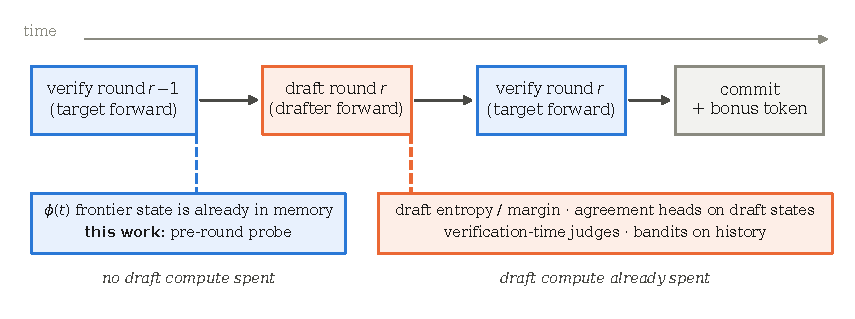
\includegraphics[width=\linewidth]{figures/fig_schematic.pdf}
\caption{Where the signal sits in the round. Checking round $r{-}1$
leaves the target's frontier state $\phi(t)$ in memory. It can be read before
round $r$'s drafter runs, so a decision made from it has spent no draft compute
at all. Each control signal we know of in prior work only becomes available
after the drafter has run, at the second dashed line.}
\label{fig:schematic}
\end{figure}


\paragraph{What this paper contributes.}
\begin{enumerate}
\item \textbf{A signal you can read before drafting.} A linear probe on the
target's cached frontier state (four layers) predicts first-token acceptance of
the coming round. It adds $+0.05$--$+0.10$ AUROC over a hard pre-round baseline
of target entropy from the round before, top-1/top-2 margin, an average of
recent acceptance, and domain. It is Platt-calibrated. Random controls of equal
capacity add nothing above chance (\S\ref{sec:results-main}).
\item \textbf{It replicates, and the test was frozen.} The result holds across
two model families and two corpora, which is three settings in all. It holds on
frozen test splits under two protocols. One is a strict dev$\to$test transfer:
the probe, scaler, fill-in values, domain list and calibrator are all frozen on
development data, and the test split is scored exactly once
(\S\ref{sec:protocol}, \S\ref{sec:results-main}).
\item \textbf{A causal check at the level of the state.} We steer the target's
state along the probe direction with forward hooks, at matched norms and graded
doses. This disrupts real acceptance $2$--$10\times$ more than random and
shuffled controls. The effect grows with dose, holds beyond the entropy change
it induces, and shows up at all four probed layers in both families
(\S\ref{sec:causal}). We call this causal evidence at the level of the state,
not a mechanistic account.
\item \textbf{Acceptance itself has shape.} Apart from any probe, an atlas of
acceptance by token category shows that tokens forced by syntax (delimiters,
operators, numbers) are accepted $+0.12$ to $+0.21$ more often than entity and
reasoning-transition tokens. This is CI-clean in all $15$ domain cells across
the three settings, on a frozen test split, against criteria we registered
before unblinding (\S\ref{sec:atlas}). The matching \emph{phase} axis does not
survive, and we report it as narrowed out.
\item \textbf{Where the signal stops.} It is first-token only. Per-length
survival probes are null to harmful at $k\ge4$, so the state does \emph{not}
support choosing run length (\S\ref{sec:length}). That sets it apart from draft
length predictors [arXiv:2412.18910]. A matched study on \emph{draft}-side
hidden states fails to beat cheap surface signals (\S\ref{sec:negatives}).
Cheap compressions of the frontier state lose most of the gain. And the
decision value is strongest where drafting is dear; within the round, entropy
control captures more of the adaptive-length headroom (\S\ref{sec:systems}).
\end{enumerate}

Taken together, these results sit in a cell that a checked sweep of the
prior work (\S\ref{sec:related}) shows is empty. That cell is: \emph{pre-round}
timing $\times$ a \emph{target-side cached} state $\times$ \emph{lossless}
exact-match SD $\times$ \emph{calibrated} odds $\times$
\emph{baseline-controlled} against free entropy, margin and history signals
$\times$ a \emph{separate} drafter $\times$ a \emph{skip-capable} decision
$\times$ a \emph{first-token} target.

\section{Related work}
\label{sec:related}

\paragraph{Work that acts once the draft has begun.} Most prior work on
speculative decoding (SD) acts after drafting starts. Stop rules read draft
entropy [arXiv:2411.18462; arXiv:2410.18351]. Learned acceptance heads read
hidden states from after the draft [arXiv:2405.19715]. Some methods schedule
the check from confidence signals sent while drafting [arXiv:2607.05147].
Others run go/stop loops on draft confidence [arXiv:2503.05096]. One line picks run lengths from
draft entropy or confidence, with compression in view [arXiv:2605.02888].
Others set the lookahead on the fly [arXiv:2405.04304], or flag drift after
the fact [arXiv:2509.01083]. A large group prunes or builds draft trees
[arXiv:2502.13652; arXiv:2402.12374; arXiv:2607.16673]. RL can tune draft
depth and check size at once [arXiv:2603.01639]. A companion model can adapt
how much text is checked [arXiv:2509.24328]. All of these read signals that
exist only once draft compute has begun. Bandits that see only past rounds
[arXiv:2505.15141] use a signal we put in our baseline.

\paragraph{Signals from the target before drafting.} AdaEAGLE
[arXiv:2412.18910] is the closest prior work. Its length predictor reads just
the signal class we use. That signal is the target's last-layer state at the
last checked spot, before the draft. But it fits draft length as a plain
number, and does not calibrate it. It is logit-free by design, so it has no
entropy or margin baseline, and it offers no skip action. It also drives a
trained EAGLE-style head [arXiv:2401.15077] rather than a drafter of its own.
Its own ablation finds that length as a class label does worse. That agrees with what we find: the
frontier state supports a first-token choice, not a choice of length. Payoff
routing for cached drafts [arXiv:2606.01019] predicts the accepted length of a
stored draft. It reads cache and history features only --- no hidden states,
no skip. Routing over drafter types from target-side signals
[arXiv:2606.07710] picks \emph{which} drafter to run. It does not ask
\emph{whether} drafting pays.

\paragraph{Judging at check time, and looser acceptance.} Judge Decoding
[arXiv:2501.19309] scores tokens that have already been drafted. It puts a
head on target embeddings, and it relaxes the lossless guarantee. Another
line probes draft and target states for semantic acceptance during the check
[arXiv:2602.03708]. That also changes the correctness contract. We do neither:
we keep the exact-match check, and we act strictly before the round.

\paragraph{Studies of acceptance, and theory.} Studies at the domain grain
[arXiv:2604.14682] record how much acceptance varies by task. We control for
that with domain one-hots. A theory of acceptance certificates
[arXiv:2606.30265] derives sharp margin-based bounds for strict greedy
acceptance. In those bounds the target's top-1/top-2 margin is the governing
term. That is why our baseline \emph{must} include margin and entropy.
Without them, our claim of added value would not mean much.

\paragraph{Probing before generation.} Linear probes read model states before
generation to predict whether an answer or a block of code will be right
[arXiv:2509.10625; arXiv:2606.14530]. We adapt that template. Other work
reports that linear directions often fail to carry across tasks
[arXiv:2506.08572]. That is why our design tests across model families and
across corpora.

\section{The setting}
\label{sec:setting}

\paragraph{How the decoding loop works.} A target model $T$ and a separate
drafter $D$ share a tokenizer and decode greedily. In round $r$, $D$ proposes
up to $L$ tokens on top of the kept prefix. $T$ checks them all in one
forward pass. The longest run that agrees with $T$'s own greedy pick is
kept, plus one bonus token. The tokens that come out are exactly the ones
$T$ would have written alone.

\paragraph{The frontier state.} This is the object the paper is about, so here
it is in words first. When $T$ checked the last round, it built an internal
state for each token in the prefix. We take that state at the last kept
token, at four depths, and join them into one long vector. That vector is what
the probe reads. It is free, because the check built it, and it is
in memory before the next round drafts.

Now in symbols. Let $x_{1:t}$ be the kept prefix after round $r{-}1$.
Checking round $r{-}1$ built $T$'s residual stream over that prefix.
Write $h_\ell(t)\in\mathbb{R}^{d}$ for the layer-$\ell$ residual-stream state at
the frontier, the last kept spot. Our candidate signal for round $r$
is the concatenation $\phi(t)=[h_{\ell}(t)]_{\ell\in\{6,12,18,24\}}$. Here
$d_{\mathrm{model}}=3584$ for the Qwen pair and $4096$ for Llama, so $\phi$ has
$14{,}336$ and $16{,}384$ dimensions. Note that $\phi(t)$ exists in memory
before round $r$ drafts.

\paragraph{What we predict.} The label is \emph{first-token acceptance}:
whether the first drafted token of round $r$ matches $T$'s greedy pick, which
is the same as an accepted length of at least $1$. For run length we use
survival labels $\mathbf{1}[A_r\ge k]$ for $k\in\{1,2,4,6,8\}$. These come from
the round's full-information record, since the engine logs agreement at each
proposed spot, whatever policy ran.

\paragraph{The bar we must beat.} Each gain we report is \emph{incremental}
over a frozen baseline. That baseline holds each free pre-round signal we
could find: (i) an average of recent acceptance over strictly earlier rounds;
(ii) the target's next-token entropy at the frontier from the round before;
(iii) the target's top-1/top-2 margin from the round before; (iv) per-column
missing flags with mean fill-in; and (v) domain one-hots. Items (ii) and (iii)
are free byproducts of the check. Certificate theory [arXiv:2606.30265] says
they carry the governing variable for greedy acceptance, so leaving them out
would make any claim of a gain meaningless. Item (v) rules out the worry that
the state merely tells us which domain we are in.

\section{How we ran the study}
\label{sec:protocol}

\paragraph{Models and corpora.} The main pair is Qwen2.5-7B-Instruct (target) /
Qwen2.5-0.5B-Instruct (drafter). The replication pair is
Llama-3.1-8B-Instruct / Llama-3.2-1B-Instruct. We pin the model revisions.
Corpus v1 has $644$ prompts over four domains: chat, code, math, and
summarization. Corpus v2 has $1{,}494$ prompts over seven axes. The new ones
here are translation, retrieval-grounded QA, and structured generation. Decode
traces are sealed sweeps. Each one has a fixed length ($L{=}8$). We set
$\mathrm{max\_new}=256$, we use bf16, and we send one request per batch. The
runs are all on A100-class hardware. We report three settings: (Qwen, v1),
(Qwen, v2), and (Llama, v1).

\paragraph{Engine validity.} In fp32 the engine passes bit-identity gates
against target-only greedy decoding. It passes them in all of the tests and in
both families --- e.g.\ $118/118$ on the Llama pair. The gates cover the skip,
stop-rule, and end-of-sequence edge cases. In bf16, the math is not exact.
Parallel-verify and sequential-decode differ at the ${\sim}0.7\%$/token level,
through argmax ties. For each request, we log whether the two paths stayed
equivalent. The acceptance labels stay exact in-context ground truth, even
when the two paths diverge.

\paragraph{Capture.} In each setting we capture $\phi(t)$ once for each round
that carries a proposal. We take it at the frontier position of that round. We
do this by teacher-forcing the target over the committed prefix. We use $400$
prompts. We draw them by domain-stratified round-robin. An early capture used
a sorted-truncation sampler. That gave us ${\sim}2$ domains per run, so we
swapped it out. All of the captures we report are stratified. Row counts are
$23{,}568$ (Qwen-v1), $14{,}122$ (Qwen-v2), and $19{,}269$ (Llama), each
$\times$ four layers. The rows are stored in fp16.

\paragraph{Splits and fitting.} All splits are prompt-grouped: 50/50 dev/test,
with a fixed seed. No split anywhere is random at the token or row level.
Probes are logistic models with an $\ell_2$ penalty ($C{=}0.1$). We chose $C$
on dev so that fits converge and repeat run to run. We saw that fits with too
little penalty depend on the BLAS thread count. Each probe is fit under
GroupKFold ($5$ folds). In each fold we standardize the columns to zero mean
and unit variance. We score each candidate against two
\emph{equal-capacity controls}. These are i.i.d.\ Gaussian columns. They have
exactly as many columns as the candidate. One set is raw. The other one is
std-matched per column. A ``lift'' that random columns of equal capacity can
match is not a lift. Error bars are 95\% prompt-grouped bootstrap CIs on
\deltaAUROC{}. We draw $1{,}000$ resamples, or $2{,}000$ for the length
probes. We report \pdle{} as well. For calibration we fit one global Platt map
on the out-of-fold scores. The map is monotone, so it keeps AUROC as it was.
The decision metrics, ECE and regret, are then scored on calibrated
probabilities.

\paragraph{Two frozen test protocols.} Work on the dev set left exactly one
candidate alive: the raw frontier state. See \S\ref{sec:negatives} for the
variants we turned down. We then scored the frozen test split once per
protocol. There was one pre-registered spec and no test-side selection:
\begin{itemize}
\item \textbf{P1, within-test OOF:} we run the dev-frozen pipeline ---
features, $C$, domain control, seed --- under prompt-grouped OOF \emph{within}
the test rows. Nothing is selected on test, but fold models are fit on test
rows.
\item \textbf{P2, strict dev$\to$test transfer:} the scaler, probe, control
columns, imputation means, domain vocabulary, and Platt calibrator are all fit
on dev only. Test rows are scored exactly once. No parameter of any kind is
fit on test.
\end{itemize}
Of the two, P2 is the deployment-faithful protocol. We report P1 so that it
can be set next to the work on the dev set. Reported numbers reproduce across
independent containers to ${\sim}{\pm}0.001$ AUROC. That spread is BLAS
reduction-order noise. It is an order of magnitude below the CI half-widths.

\section{Results}
\subsection{The target's cached state predicts next-round acceptance}
\label{sec:results-main}

Table~\ref{tab:dev} gives the results on the dev split, with domain held
fixed. Table~\ref{tab:frozen} gives the frozen-test results from the one-shot
run, under both protocols. The pattern is the same in all three settings. The
frontier state adds $+0.04$--$+0.11$ AUROC on top of the hardened baseline.
The CIs exclude zero, with $\pdle=0.000$. Controls with equal capacity sit at
or below the baseline. Their AUROCs are $0.53$--$0.56$. That is, the added
random columns buy us nothing. The lift is information, not capacity.



\begin{table}[t]
\centering
\caption{Development split. Gain from the frontier state over the
pre-round baseline of entropy, margin, history and domain, with domain
controlled. Prompt-grouped OOF; 95\% grouped-bootstrap CIs; $\pdle=0.000$ for
all three settings.}
\label{tab:dev}
\begin{tabular}{lcccc}
\toprule
Setting & \#domains & Baseline AUROC & Combined AUROC & \deltaAUROC \\
\midrule
Qwen-v1 & 4 & 0.670 & 0.742 & $+0.072$ \\
Qwen-v2 & 7 & 0.618 & 0.731 & $+0.112$ \; {\footnotesize[+0.095, +0.130]} \\
Llama-v1 & 4 & 0.696 & 0.765 & $+0.069$ \\
\bottomrule
\end{tabular}
\end{table}





\begin{table}[t]
\centering
\caption{One-shot frozen \textbf{test} results for a single candidate
registered in advance. P1 scores within the test split. P2 is the strict
dev$\to$test transfer, with nothing at all fit on test. In each cell
$\pdle=0.000$, and the combined model beats both equal-capacity controls. The
control column gives the best control AUROC under P2.}
\label{tab:frozen}
\begin{tabular}{lccccc}
\toprule
Setting & $n_{\mathrm{test}}$ & P1 \deltaAUROC{} [95\% CI] &
P2 \deltaAUROC{} [95\% CI] & P2 Base$\to$Comb & P2 Ctrl \\
\midrule
Qwen-v1 & 11{,}982 & $+0.076$ {\footnotesize[+0.063, +0.089]} &
$+0.056$ {\footnotesize[+0.041, +0.070]} & $0.660\to0.716$ & 0.542 \\
Qwen-v2 & 7{,}191 & $+0.092$ {\footnotesize[+0.073, +0.111]} &
$+0.103$ {\footnotesize[+0.083, +0.124]} & $0.626\to0.729$ & 0.528 \\
Llama-v1 & 9{,}610 & $+0.053$ {\footnotesize[+0.037, +0.070]} &
$+0.039$ {\footnotesize[+0.023, +0.057]} & $0.713\to0.752$ & 0.559 \\
\bottomrule
\end{tabular}
\end{table}






\begin{figure}[t]
\centering
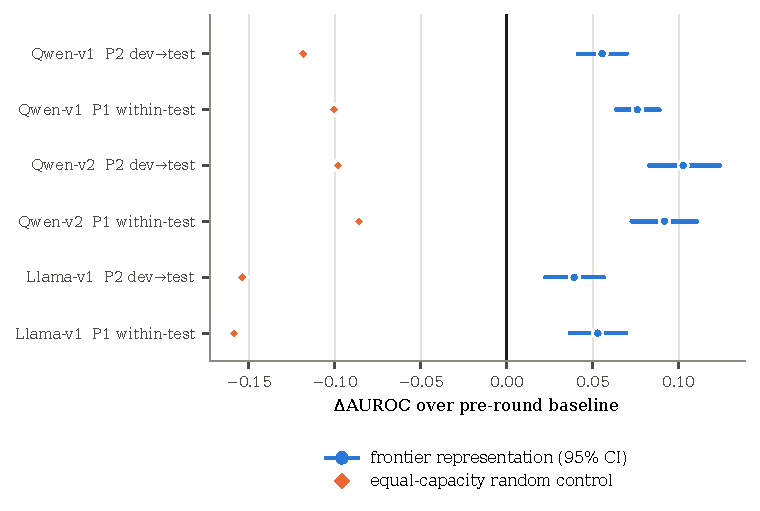
\includegraphics[width=0.72\linewidth]{figures/fig_forest.pdf}
\caption{Gain from the frontier state over the pre-round baseline on
the frozen test split, for both protocols and all three settings (95\%
grouped-bootstrap CIs; each interval clears zero, $\pdle=0.000$). Diamonds show
what the equal-capacity random control adds over the same baseline. Adding the
same number of random columns does not just fail to help. It drags the model
down to near chance (control AUROC $0.53$--$0.56$). So the blue intervals
measure information, not size.}
\label{fig:forest}
\end{figure}



The baseline holds domain one-hots, and the captures are split by domain. So
the lift is not the probe telling domains apart. The baseline also holds the
target's entropy and margin from the round before. In theory, those two are
the free variables that drive the outcome [arXiv:2606.30265]. So the result
says this: \emph{Entropy and margin are not a sufficient statistic for
pre-round acceptance. The cached state holds more that bears on the choice.}

\subsection{Calibration}
\label{sec:calibration}



\begin{figure}[t]
\centering
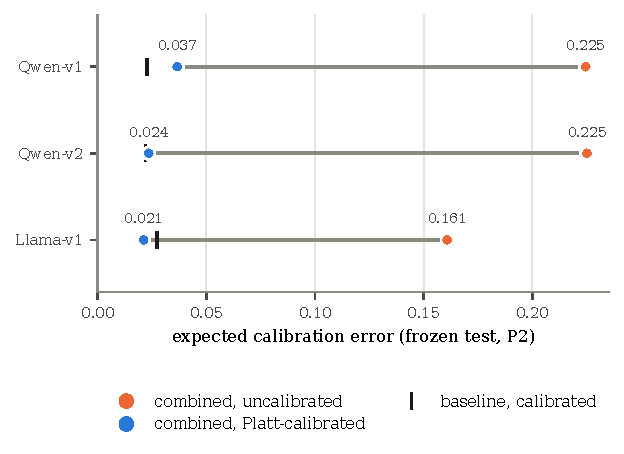
\includegraphics[width=0.66\linewidth]{figures/fig_calibration.pdf}
\caption{How honest the stated odds are, on the frozen test split
under the strict protocol. The raw probe is far too sure of itself. One global
Platt map pulls it back to the baseline's level and leaves its ranking alone.
Tick marks show the calibrated baseline for reference. Note that this is a
summary of one number per setting, not a reliability diagram, because the
sealed artifacts record only the aggregate ECE.}
\label{fig:calibration}
\end{figure}




Raw probes over many dimensions are too sure of themselves. Before
calibration, the combined ECE runs as high as $0.14$. One global Platt map
fixes most of that. The map keeps AUROC, and it is safe from leaks. It brings
the test ECE back to $0.016$--$0.024$ under P1. Under P2 we freeze the map on
dev OOF scores. We then apply it to test scores from a model fit on all of
dev. That shift in the spread of scores costs us some calibration quality on
one setting. The combined test ECE is $0.037$ on Qwen-v1 and $0.024$/$0.021$
on v2/Llama. We report that, rather than patch it after the fact. The ranking
metrics do not change.

\subsection{The signal is first-token only}
\label{sec:length}

Per-length survival probes $P(A\ge k)$ (Table~\ref{tab:length}) show where the
signal sits. The lift is strong and CI-clean at $k{=}1$ in all three settings.
At $k\ge4$ it is null to \emph{harmful}. It is significantly worse than the
baseline on v2/Llama at $k{=}8$. That is the point where domain and history
already predict long runs. A length controller run off the survival probe
likewise fails to beat one run off the baseline. The one exception is a small
win at a single draft-cost point. The frontier state answers ``will
speculation connect at all next round?''---not ``for how long?''. That marks a
clean split from pre-draft \emph{length} regression [arXiv:2412.18910]. Its
own ablations show that classing by length does worse. It also points to the
skip/admission choice as the natural user of the signal.



\begin{table}[t]
\centering
\caption{Gain by run length, \deltaAUROC{} (development split, domain
controlled, $2{,}000$-resample grouped bootstrap). Bold marks a CI-clean gain.
``worse'' marks a CI-clean loss.}
\label{tab:length}
\begin{tabular}{lccc}
\toprule
$k$ & Qwen-v1 & Qwen-v2 & Llama-v1 \\
\midrule
1 & $\mathbf{+0.073}$ & $\mathbf{+0.103}$ & $\mathbf{+0.065}$ \\
2 & $+0.008$ (null) & $\mathbf{+0.045}$ & $-0.007$ (null) \\
4 & $-0.010$ (null) & $-0.004$ (null) & $-0.019$ (worse) \\
6 & $-0.002$ (null) & $-0.011$ (null) & $-0.032$ (worse) \\
8 & $+0.002$ (null) & $-0.018$ (worse) & $-0.021$ (worse) \\
\bottomrule
\end{tabular}
\end{table}






\begin{figure}[t]
\centering
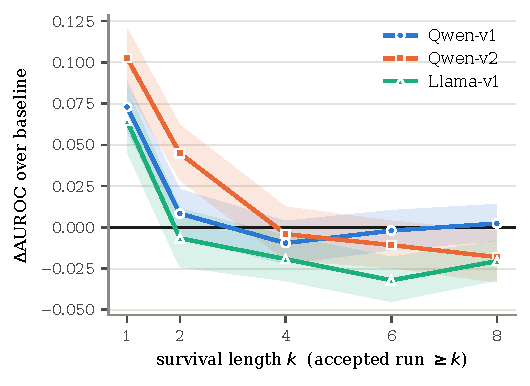
\includegraphics[width=0.55\linewidth]{figures/fig_length.pdf}
\caption{Gain by run length (development split, domain-controlled;
bands are 95\% grouped-bootstrap CIs). The whole signal sits at $k{=}1$. By
$k{=}4$ it has fallen to zero or below in all three settings. In short, the
frontier state tells you whether speculation will connect, not how far it will
run.}
\label{fig:length}
\end{figure}



\subsection{Steering the direction disrupts acceptance}
\label{sec:causal}




\begin{figure}[t]
\centering
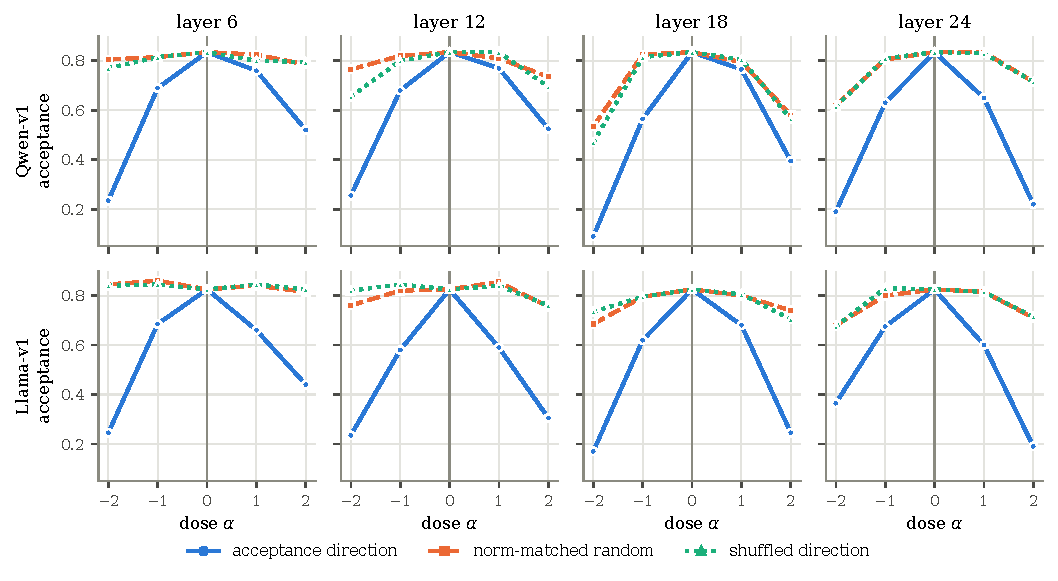
\includegraphics[width=\linewidth]{figures/fig_dose.pdf}
\caption{What happens when we steer the target's frontier state, at all
four probed layers, in both families we ran interventions on. Qwen-v2 was never
steered, so it has no panel here. Steering along the fitted acceptance
direction drives real acceptance down, and harder doses do more damage, giving
an upside-down U that peaks at $\alpha{=}0$. Random and shuffled directions at
the same norm and the same dose stay nearly flat.}
\label{fig:dose}
\end{figure}



A lift in what we can predict is not enough on its own. It cannot tell a
load-bearing state from a mere shadow. So on held-out test rounds we steer the
target's residual stream at the frontier spot. We do this with forward hooks:
$h_\ell \leftarrow h_\ell + \alpha\,\sigma_\ell\,\hat d_\ell$. Here
$\hat d_\ell$ is the first-token acceptance direction fit on dev. Next,
$\sigma_\ell$ is the mean frontier-state norm, which sets a natural dose
scale. The dose itself is $\alpha\in\{-2,-1,0,+1,+2\}$. Each layer gets
controls: random directions matched on norm, and shuffled ones. A no-op check
confirms the hook site (fidelity $0.95$ Qwen-v1 / $1.00$ Llama). Steering
along $\hat d_\ell$ disrupts measured first-token acceptance $2$--$10\times$
more than the matched controls. The size of the hit tracks the dose
(inverted-U peaking at $\alpha{=}0$). It holds at all four probed layers, and
in both families. On Llama the real hit is $0.32$--$0.40$, while the controls
are ${\approx}0$. The gap between real and control holds up even in narrow
bins of the induced entropy change. So the effect is not routed through
entropy alone. We read this strictly at the representation level. The probed
direction causally drives whether the target's next token can agree. We make
no claim about the inner computing structure.

\subsection{What it costs, and where it matters}
\label{sec:systems}



\begin{figure}[t]
\centering
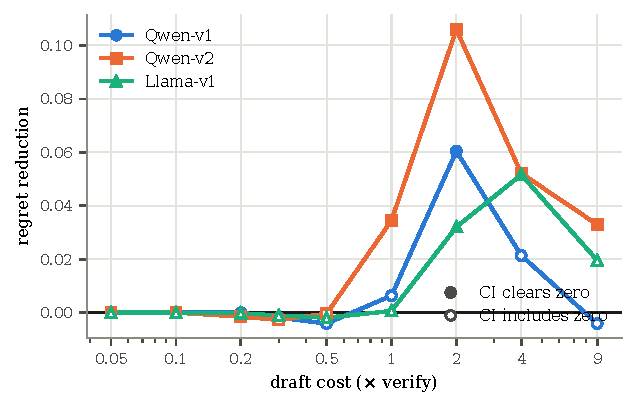
\includegraphics[width=0.66\linewidth]{figures/fig_regret.pdf}
\caption{Whether the pre-round signal changes a real decision as draft
cost varies (frozen test, strict protocol; higher is better). Filled markers
are the costs where the recorded CI clears zero. While drafting is cheap the
signal does nothing, because each calibrated model just picks ``always
draft''. It starts to pay only once draft cost nears or passes check cost.
Qwen-v1 clears the CI bar at a single cost point, which is the protocol
sensitivity we report in the text.}
\label{fig:regret}
\end{figure}




\paragraph{Cost.} Reading $\phi(t)$ is free on the capture path, since the
states fall out of the check anyway. The probe is one $14$k-dimensional dot
product. That takes ${\sim}16\,\mu s$ per round on our setup, or
${\sim}0.015\%$ of a decode round. The honest caveat is about engineering, not
compute. Serving engines do not keep frontier states from many layers today.
To ship this, one must expose them (cheap) or find a compact sufficient
statistic (open; \S\ref{sec:negatives}).

\paragraph{Decision proxy.} We sweep a calibrated skip/draft choice across
draft-cost ratios. When drafting is cheap ($\le0.2\times$ verify), every
calibrated model picks ``always draft''. No pre-round signal changes any
choice there. That fits our finding that adding a skip arm under cheap serving
costs \emph{hurts} ($-0.3$ to $-0.7\%$). At a draft cost of $\ge 1\times$
verify, the cut in regret from the probe is CI-robust. That holds across a
range of costs on Qwen-v2 and Llama, under both protocols. Under P1 it holds
on Qwen-v1 as well. Under P2 it is CI-robust only at one cost---a protocol
sensitivity we report. So the pre-round signal is relevant to the decision
where drafting is costly: launch-bound drafters, large drafters, and packed
batch serving. Elsewhere it is diagnostic.

\paragraph{Where pre-round control fits.} For adaptive \emph{length}, a
within-round draft-entropy stop is still stronger. It beats the best fixed
length by $+6.7$--$+11.2\%$ serving-efficiency across our three settings (as
one example, $+11.2\%$, 95\% CI $[+10.3\%, +12.1\%]$ on Qwen-v1). A pre-round
frontier-entropy gate wins back only ${\sim}1/3$--$1/2$ of that gain. The two
signals pair up by timing. One is
pre-round admission/skip and scheduling. The other is within-round stopping.

\subsection{Negative results that back the claim}
\label{sec:negatives}

Three negative results sharpen the claim.

(i) \emph{Draft-side hidden states do not beat surface signals.} On the same
traces, we ran a matched study of what each part adds. A linear probe on the
\emph{drafter's} residual stream (best layer) reaches $0.803$ AUROC. A surface
stack of entropy, margin, history, and position reaches $0.870$. Adding the
probe to that stack gains at most $+0.006$. So the pre-round result is not
``probes beat baselines'' in general. It is the target-side, pre-round framing
that does the work.

(ii) \emph{Cheap compressions lose the signal.} Low-rank projections
($k{=}16$), norm summaries, layer-alignment features, and drift speeds add
only $+0.01$--$+0.04$. They are also not stable across settings. Only the full
state clears the bar in all three. A compact sufficient statistic is the main
open question for engineers.

(iii) \emph{History-only control is weak.} The EMA of acceptance history is
already in our baseline. Stationary bandit controllers over length arms
[arXiv:2505.15141] learn the best single arm. By design, they thus tie the
best fixed length in our replays. Serving-efficiency is $2.4015$ for them and
$2.4022$ for best-fixed. The contextual entropy stop reaches $2.6715$. That is
context, not a contest, for signals at the representation level.

\section{What acceptance is about}
\label{sec:atlas}

The sections up to here show that a pre-round signal exists, and that it is
causally load-bearing. This section asks a second kind of question, and it is
a purely \emph{behavioral} one. We use no probes here, and we look at no inner
states. We just ask whether acceptance itself has a shape we can read.

We answer with an \emph{acceptance atlas}. The atlas is the rate of
acceptance, split by token category and by phase of generation. We build it
from the same sealed traces we used above, and we put prompt-grouped bootstrap
CIs on each cell. The labels come from the counterfactual record of what the
target would have done at each position. The categories come from version
v1.0.0 of the overlapping taxonomy. The phase bins are set by absolute
position.

\paragraph{Domain control.} Our domain marginals match the domain-grain
acceptance axis reported before [arXiv:2604.14682]. Here is one case of that,
on Qwen-v1 dev: summarization $0.657 <$ chat $0.700 <$ code $0.813 <$ math
$0.875$. We treat that axis as a \emph{control}, and our pipeline does recover
it. What we add is the finer structure inside a domain. That structure sits at
the category level, and it is still there once we condition on the domain.

\subsection{Structural tokens are accepted far more often than entity tokens}
\label{sec:atlas-contrast}

We pre-registered one contrast on dev data. It was HIGH
(\texttt{code\_delimiter}, \texttt{operator}, \texttt{number}, pooled) minus
LOW (\texttt{named\_entity}, \texttt{reasoning\_transition}, pooled). At the
same time we fixed the criteria T1--T4 and the rule that maps each one to an
outcome. We wrote all of that down and committed it before the test split was
unblinded. Table~\ref{tab:atlas} gives the one-shot test result. A script did
the scoring, so each verdict comes from those criteria just as we had
committed them.



\begin{table}[t]
\centering
\caption{One-shot frozen \textbf{test} check of the acceptance atlas
against criteria we registered before unblinding. T1: the overall HIGH$-$LOW
contrast. T2: is that contrast positive and CI-clean inside each domain cell.
T3: do the tails stay stable against the setting's overall rate. T4: the phase
spread (max$-$min), registered in advance as an expected null on the Qwen
settings. PASS 3/3.}
\label{tab:atlas}
\begin{tabular}{lccc}
\toprule
Criterion & Qwen-v1 & Qwen-v2 & Llama-v1 \\
 & {\footnotesize(152{,}592 tok)} & {\footnotesize(209{,}160)} &
 {\footnotesize(124{,}000)} \\
\midrule
T1 overall contrast & $+0.1947$ & $+0.2104$ & $+0.1177$ \\
 & {\footnotesize[+0.172, +0.216]} & {\footnotesize[+0.193, +0.228]} &
 {\footnotesize[+0.103, +0.134]} \\
 & {\footnotesize$\pdle=0$} & {\footnotesize$\pdle=0$} &
 {\footnotesize$\pdle=0$} \\
T2 within-domain & 4/4 CI-clean & 7/7 CI-clean & 4/4 CI-clean \\
T3 tail stability & PASS {\footnotesize(marg.\ 0.742)} &
PASS {\footnotesize(0.688)} & PASS {\footnotesize(0.833)} \\
T4 phase spread & $0.0084$ PASS & $0.0036$ PASS &
$0.0589$ {\footnotesize(descr.)} \\
\bottomrule
\end{tabular}
\end{table}






\begin{figure}[t]
\centering
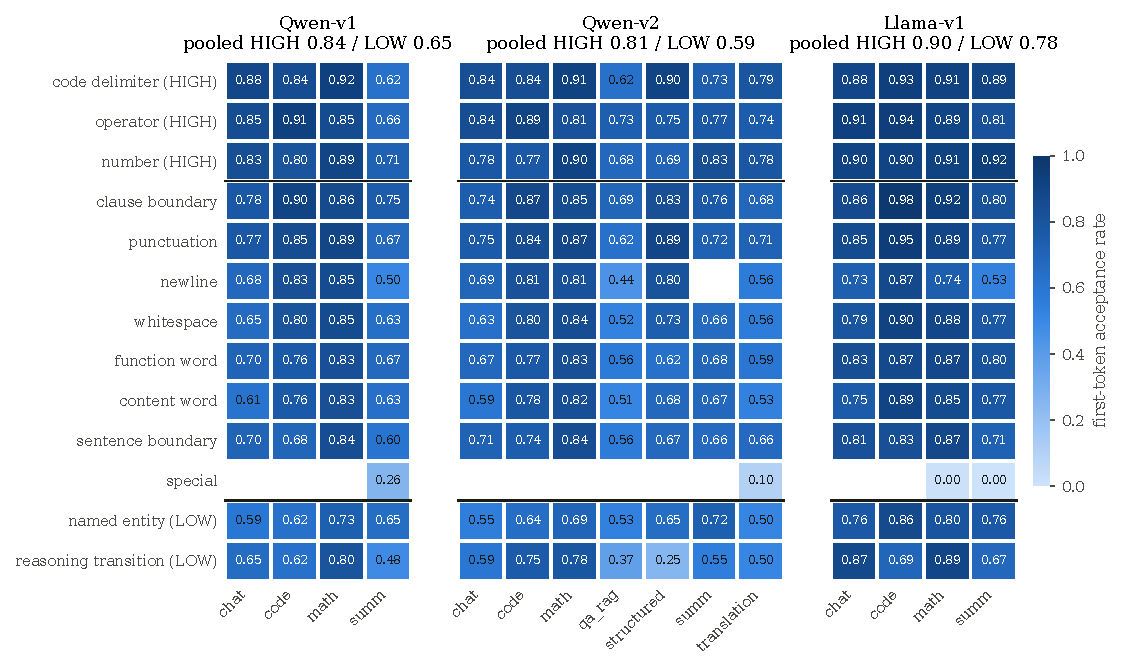
\includegraphics[width=\linewidth]{figures/fig_atlas.pdf}
\caption{The acceptance atlas on the frozen test split. Each cell is the
first-token acceptance rate for one token category (rows) inside one domain
(columns), with one panel per setting. Rows are grouped by the pools we
registered in advance: the HIGH block sits on top, the LOW block below the
rule. Blank cells hold too few tokens to report. The key point is that
structural tokens beat entity tokens inside each domain of each setting, not
just in the totals. The Llama \texttt{special} row ($\approx 0.00$) is the
template-handling oddity noted in \S\ref{sec:atlas-phase}, and it is left out
of the contrast.}
\label{fig:atlas}
\end{figure}



The contrast is large: it runs from $+0.12$ to $+0.21$ in acceptance. And it
is not domain identity in disguise. It is CI-clean positive in \emph{all 15}
of the domain cells, across the three settings. The tails of the category
order are stable across the families as well. In every setting,
\texttt{code\_delimiter}, \texttt{operator}, \texttt{number},
\texttt{clause\_boundary}, and \texttt{punctuation} sit above the marginal. In
every setting, \texttt{named\_entity} sits below it. The reading of this is a
plain one: a small drafter is good at the tokens that syntax forces on the
spot. It misses the tokens that call for what the target knows, or for a
choice the target has to make. \texttt{reasoning\_transition} is low on the
Qwen pair only.

We owe the reader two disclosures. First, the \emph{expected null} that we had
set in advance came out positive. Llama-code was flat on dev, at $-0.006$, and
it sat at a $0.913$ acceptance ceiling. We had named it in advance as a cell
that was free to be null. But on test it came in at $+0.0674$
{\footnotesize[+0.0304, +0.1097]}. So the null we saw on dev was just noise
from that ceiling. Second, the weakest cell that survives is Qwen-v1
summarization. It comes in at $+0.0544$, with $\pdle=0.027$ and a percentile
CI lower bound of $-0.002$. That clears the $p<0.05$ bar we had set in
advance. We flag it as the one margin to watch in any re-run.

\subsection{The phase axis does not survive}
\label{sec:atlas-phase}

The claim as we first posed it had a second half. That half said acceptance
would vary across the phases of generation, and it did not survive. On both
Qwen settings the phase spread is flat on test, and flat by a wide margin. The
two values are $0.0084$ and $0.0036$, against a bar of $\le 0.03$ that we had
set in advance. Here the bins are set by absolute position.

The Llama pair does show a rise that is monotone: prefix $0.794 \to$ mid
$0.824 \to$ late $0.853$. But that is one family on its own, and a length or
mix confound is plausible. So we record the rise descriptively, and we make no
claim from it. We therefore narrow the atlas result to the category axis, and
to that axis only. Phase bins set by absolute position carry no acceptance
structure that holds across the families at this grain.

One more descriptive oddity, which we record but do not explain. On the Llama pair the
\texttt{special} category accepts at $0.007$ ($n{=}883$). The most likely
cause is not an acceptance effect. It is a gap in how the two pairs handle
chat templates and special tokens. We leave it out of the contrast, and we
flag it for work of its own.

\section{Limitations}
\label{sec:limitations}

Each item below sets a bound on what we claim.

\begin{itemize}

\item We look at the first token, and at the first token only. We make no
claim about run length. The length-aware controller does not benefit.

\item We use the full frontier state. A cheap variant that is ready to deploy
is still open.

\item We test only one mode of speculative decoding: greedy exact match.
Acceptance under sampling is untested.

\item We use two model families. We use one drafter in each family.
Speculators with a trained head (EAGLE-class) are out of scope by design. Ours
is the cell in which the drafter is independent.

\item We picked layers $\{6,12,18,24\}$ for the depth of the drafter. We then
used the same layers for the deeper targets. A layer sweep tuned to the target
may make the result stronger. It may also localize it.

\item The decision analysis is a proxy. It is calibrated. It runs over sealed
traces. We did not run the end-to-end wall-clock test with the probe in the
serving path---that test is our systems gate. So we make no wall-clock claim.

\item We run a batch-size-1 harness. We did not measure how batches interfere
with each other.

\item Under the strict protocol, calibration gets worse on one setting. We
report that.

\item We describe the bf16 argmax-tie trajectory divergence, and we log it. We
do not remove it.

\item The atlas (\S\ref{sec:atlas}) is narrow. It uses one taxonomy of
categories, and they overlap. We use version v1.0.0 of that taxonomy. The
labels it uses are counterfactual. They mark agreement over a fixed length.
The atlas covers two model families and two corpora. Its phase half is
narrowed out. That half is not supported. The atlas is a description of
behavior only. We do not link it to the evidence inside the probe.

\end{itemize}

\section{Conclusion}
Before we spend any draft compute, the target has already cached its frontier
state. That state holds a signal, and the signal is calibrated and causally
load-bearing. It is about the first token only, not the rest of the round. It
tells us if the next round of speculation will connect. It holds up even when
we account for entropy, margin, history, and domain. It shows up in two model
families and on two corpora. All of this held under frozen-test discipline.

We offer it as an honest diagnostic, and we map its bounds precisely. It is a
signal that says whether to admit a round, and it runs before the round starts.
It adds to within-round control and does not take its place. It matters for the
decision exactly where drafting is expensive. We claim no more than that.

The last result stands on its own, with no appeal to internal states.
Acceptance itself turns out to be shaped by token category, and the effect is
strong. At the grain we tested, it is not shaped by generation phase.

\section*{Reproducibility statement}
Every number we report comes from a script, and the scripts read sealed decode
traces and activation captures. Those files are locked and do not change. No
number is worked out by hand. Splits are prompt-grouped, and the seeds are
fixed. We pre-registered the frozen-test protocol. There was one spec, and the
pass rules were fixed before we unblinded it. We ran the test once, as that
spec laid out, and we keep the first-pass artifacts next to any re-runs. In a
new container, the headline numbers hold to within ${\pm}0.001$ AUROC. The
code, the sealed artifacts, and the full claims ledger are ready for release
under a staged policy. The ledger lists all negative results and two integrity
disclosures.

\section{Terms used in this paper}
\label{sec:terms}

This reference section defines each term the paper uses. It collects in one
place the definitions the body relies on.

\begin{description}

\item[Speculative decoding (SD)] A way to make a large model write faster. A
small model guesses the next few tokens. The large model then checks all of
them in one pass. Good guesses are kept, so one pass yields several tokens.

\item[Target] The large model. It owns the output. Each token the system
emits is a token the target would have written on its own.

\item[Drafter] The small, cheap model that guesses. In this work the drafter is
a separate model, not a head bolted onto the target. It shares the target's
tokenizer.

\item[Lossless (exact-match) decoding] The output is exactly what the target
would have written by itself. Speed goes up. The text does not change. Each
result here is lossless.

\item[Round] One cycle of the loop: the drafter proposes up to $L$ tokens, the
target checks them, and the agreed tokens are kept.

\item[Acceptance] Whether a drafted token survives the check. A token is
accepted when it matches what the target would have picked at that spot.

\item[First-token acceptance] Whether the \emph{first} drafted token of a round
is accepted. This is what our probe predicts. It is a yes/no question about one
token, not a guess at how many tokens will survive.

\item[Accepted run length] How many drafted tokens in a row are accepted in a
round. Our signal does \emph{not} predict this. That limit is a main finding,
not an oversight.

\item[Frontier state] The signal this paper is about. When the target checks a
round, it computes an internal state for each token it reads. We take that
state at the last kept token, which we call the frontier. We take it at
four depths in the target (layers $6$, $12$, $18$ and $24$) and join them into
one long vector. That gives $14{,}336$ numbers for the Qwen pair and
$16{,}384$ for the Llama pair. Three points matter. It is the \emph{target's}
state, not the drafter's. It is free, because the check that just ran already
built it. And it sits in memory \emph{before} the next round drafts, which
is why we can act on it early.

\item[Probe] A simple linear model that reads the frontier state and outputs a
score for how likely the next drafted token is to be accepted. It is one dot
product. It is not a neural network.

\item[Baseline (the bar)] The set of cheap signals a probe must beat to be
worth anything. Ours holds the target's entropy and top-1/top-2 margin from the
round before, a running average of recent acceptance, and the task domain. We
made this bar deliberately hard, because a signal that only beats a weak bar
tells you nothing.

\item[Development split and test split] We cut the data in two by prompt, never
by token. We built and chose everything on the development split. The test
split was scored once, at the end, to check the result.

\item[AUROC] A score for how well a model ranks. It runs from $0.5$ to $1.0$.
A model at $0.5$ ranks no better than a coin flip. A model at $1.0$ ranks each
accepted token above each rejected one. We report the \emph{gain} in AUROC
over the baseline, so $+0.05$ means the probe adds that much on top of the bar.

\item[ECE (expected calibration error)] How honest the stated odds are. If a
model says $70\%$ and is right $70\%$ of the time, its error is zero. Lower is
better.

\item[Calibration and the Platt map] Raw probe scores rank well but state the
odds badly. A Platt map is a small correction that fixes the odds without
changing the ranking, so AUROC is untouched.

\item[Regret] What a decision costs compared with the best choice you could
have made. We use it to ask whether the signal changes any real decision, not
just whether it scores well.

\item[Equal-capacity control] A fake signal with the same number of columns as
the real one, filled with random noise. If the real signal wins only because it
is large, the control wins too. Ours do not, so the gain is information rather
than size.

\item[Protocol P1] The test rows are scored using folds fit within the test
split itself. Nothing is chosen on test, but models do see test rows.

\item[Protocol P2] The strict one. The probe, the scaler, the fill-in values,
the domain list and the calibrator are all frozen on development data. Test
rows are scored exactly once. No part of the model ever touches test data. This
is the protocol that matches deployment.

\end{description}

\begin{thebibliography}{99}
\small
% Full bibliographic entries (authors, titles, venues-as-dates) to be
% completed at submission; identifiers are primary-source verified.
\bibitem{leviathan} Fast inference from transformers via speculative decoding.
arXiv:2211.17192.
\bibitem{chen} Accelerating large language model decoding with speculative
sampling. arXiv:2302.01318.
\bibitem{eagle} EAGLE: speculative sampling with a feature-level
autoregressive head. arXiv:2401.15077.
\bibitem{specdecpp} SpecDec++: trained acceptance head on post-draft hidden
states. arXiv:2405.19715.
\bibitem{svip} SVIP: draft-entropy dynamic draft length. arXiv:2411.18462.
\bibitem{adaedl} AdaEDL: entropy-based early draft stopping. arXiv:2410.18351.
\bibitem{banditspec} BanditSpec: bandit selection of speculative-decoding
configurations. arXiv:2505.15141.
\bibitem{disco} DISCO: dynamic speculation lookahead. arXiv:2405.04304.
\bibitem{dsde} DSDE: post-hoc divergence diagnostics for speculation length.
arXiv:2509.01083.
\bibitem{c2t} C2T: classifier-based token-tree pruning. arXiv:2502.13652.
\bibitem{sequoia} Sequoia: hardware-aware token-tree optimization.
arXiv:2402.12374.
\bibitem{ltd} Learning to draft: RL coordination of draft and verification.
arXiv:2603.01639.
\bibitem{speckv} SpecKV: adaptive speculation length under KV compression.
arXiv:2605.02888.
\bibitem{adaspec} AdaSpec (ex-SpecServe): draft-confidence continue/stop
control. arXiv:2503.05096.
\bibitem{dspark} DSpark: confidence-scheduled verification in production
serving. arXiv:2607.05147.
\bibitem{sv} Speculative verification: companion-model verification-length
adaptation. arXiv:2509.24328.
\bibitem{specla} SpecLA: speculative decoding for linear-attention targets.
arXiv:2607.16673.
\bibitem{adaeagle} AdaEAGLE: pre-draft draft-length prediction with adaptive
draft structures. arXiv:2412.18910.
\bibitem{hvd} Hybrid verified decoding: cache-draft payoff routing.
arXiv:2606.01019.
\bibitem{whiflash} WhiFlash: pre-draft drafter-paradigm routing.
arXiv:2606.07710.
\bibitem{judge} Judge decoding: verification-time judgment on target
embeddings. arXiv:2501.19309.
\bibitem{semanticspec} SemanticSpec: semantic-acceptance probing during
verification. arXiv:2602.03708.
\bibitem{dynamics} Acceptance dynamics across cognitive domains.
arXiv:2604.14682.
\bibitem{theory} When is a draft accepted? A theory of acceptance in
speculative decoding. arXiv:2606.30265.
\bibitem{qprobes} Question-only probes of pre-generation activations for
answer correctness. arXiv:2509.10625.
\bibitem{codeprobes} Pre-generation hidden-state probes of code correctness.
arXiv:2606.14530.
\bibitem{truthgeom} Task-orthogonal geometries of linear truth directions.
arXiv:2506.08572.
\end{thebibliography}

\end{document}
